\documentclass[12pt,a4paper,twoside]{article}
\usepackage{geometry}
\geometry{a4paper}

\usepackage{pgfplots} %wykresy
\usepackage[utf8]{inputenc}
\usepackage[OT1]{fontenc}
\usepackage{graphicx} %wstawianie obrazków
\usepackage{epstopdf} %wstawianie obrazków w formacie .eps
\usepackage{setspace}
\usepackage{fancyhdr} %nagłówki i stopki na każdej stronie
\usepackage{amsmath}
\usepackage{amssymb}
\usepackage{enumitem}
\usepackage{microtype}
\usepackage{url}
\usepackage{floatrow} %domyślnie wyśrodkowuj ryciny
\usepackage[english,polish]{babel}
\usepackage{polski}
\usepackage{mathtools} %\ceil, \floor
\usepackage[title]{appendix} %appendices
\usepackage{caption} %multi-line caption
\usepackage{siunitx} %separatory w dużych liczbach
\usepackage{fancyvrb} %centrowanie verbatimów

\pgfplotsset{compat=1.5} %wersja biblioteki do wykresów; usuwa problemy
\newcounter{wlcounter} %licznik list słów

\begin{document}
\newgeometry{margin=3cm}
\onehalfspacing
\newcommand{\myparagraph}[1]{\paragraph{#1}\mbox{}\\}
\newcommand{\latin}[1]{\foreignlanguage{latin}{\textit{#1}}}
\newcommand{\en}[1]{\textit{\enn{#1}}}
\newcommand{\enn}[1]{\foreignlanguage{english}{#1}}
\newcommand{\abbr}[1]{\textit{#1}}
\newenvironment{myenumerate}
    {\begin{enumerate}[label*=\arabic*.]}
    {\end{enumerate}}
\DeclarePairedDelimiter{\ceil}{\lceil}{\rceil}
\DeclarePairedDelimiter{\floor}{\lfloor}{\rfloor}

\begin{titlepage}
    \begin{center}
    {\LARGE Uniwersytet im. Adama Mickiewicza w~Poznaniu \\
    Wydział Matematyki i~Informatyki}
    \line(1,0){350}

    \vspace{1cm}
    
\includegraphics[width=2cm]{logo-uam/logo-uam.png}
    \vspace{1cm}

    \vspace{1cm}
    {\Huge Ataki na kryptograficzne \\ funkcje skrótu} \\[0.5cm]
    {\Large Marcin Kurczewski}
    \end{center}

    \vspace{3cm}
    \hspace{8cm}\parbox[l]{6cm}{\Large Praca magisterska \\
    napisana pod kierunkiem \\
    dr Michała Rena}

    \begin{center}
    \vspace{4cm}
    Poznań, maj 2013
    \end{center}
\end{titlepage}


\newpage
\thispagestyle{empty}
\begin{center}
    OŚWIADCZENIE
\end{center}

Ja, niżej podpisany Marcin Kurczewski, student Wydziału Matematyki
i~Informatyki Uniwersytetu im. Adama Mickiewicza oświadczam, że przedkładaną
pracę dyplomową pt.: ``Ataki na kryptograficzne funkcje skrótu'' napisałem
samodzielnie. Oznacza to, że przy pisaniu pracy, poza niezbędnymi
konsultacjami, nie korzystałem z~pomocy innych osób, a~w~szczególności nie
zlecałem opracowania rozprawy lub jej części innym osobom, ani nie odpisywałem
tej rozprawy lub jej części od innych osób.

Oświadczam również, że egzemplarz pracy dyplomowej w~formie wydruku
komputerowego jest zgodny z~egzemplarzem pracy dyplomowej w~formie
elektronicznej.

Jednocześnie przyjmuję do wiadomości, że gdyby powyższe oświadczenie okazało
się nieprawdziwe, decyzja o~wydaniu mi dyplomu zostanie cofnięta.


\newpage
\setcounter{tocdepth}{3}
\tableofcontents

\newpage
\pagestyle{fancy}
\fancyhead[L]{\fontsize{10}{0}\selectfont
    Ataki na kryptograficzne funkcje skrótu}
\fancyhead[R]{\fontsize{10}{0}\selectfont
    Marcin Kurczewski}


\section{Wstęp}
Celem tej pracy jest przedstawienie współczesnych metod łamania
kryptograficznych funkcji skrótu, zarówno od strony praktycznej, jak
i~teoretycznej. Jako główny temat technologiczny zostały wybrane funkcje
\texttt{MD5} oraz \texttt{SHA-1}.

Praca złożona jest z~trzech części. Pierwsza stanowi wprowadzenie do tematyki
kryptograficznych funkcji skrótu, opisując krótko ich rys historyczny,
zgłębiając szczegółowo budowę i~przedstawiając ich zastosowania.

Druga część opisuje szereg uniwersalnych technik, które można zastosować do
atakowania większości współczesnych kryptograficznych funkcji skrótu w~sposób
niezależny od ich struktury. W~części tej są także przedstawione podstawowe
metody obrony przed tego typu atakami.

Część trzecia prezentuje od strony technicznej wybrane wysoce wyspecjalizowane
ataki teoretyczne, jakie powstały na przestrzeni ostatnich lat, pokazując luki
w~kryptograficznych funkcjach skrótu.

\newpage



\section{Wprowadzenie do tematyki}



\subsection{Terminologia użyta w~pracy}
Zgodnie z~terminologią stosowaną w~kryptologii, w~pracy konsekwentnie
wykorzystywane będą następujące pojęcia:

\begin{itemize}

    \item \textbf{funkcja haszująca}~-- alternatywne określenie na
    \emph{funkcję skrótu},

    \item \textbf{bezpieczna funkcja haszująca}~-- alternatywne określenie na
    \emph{kryptograficzną funkcję skrótu},

    \item \textbf{zwykła funkcja haszująca}~-- funkcja skrótu, która może, ale
    nie musi być \emph{kryptograficzną funkcją skrótu},

    \item \textbf{wiadomość}~-- wartość wejściowa dla \emph{funkcji skrótu},

    \item \textbf{skrót}~-- wartość wyjściowa z~\emph{funkcji skrótu},

    \item \textbf{hasz}~-- alternatywne określenie na wartość wyjściową
    \emph{funkcji skrótu},

    \item \textbf{kolizja}~-- sytuacja, w~której skróty dwóch różnych
    wiadomości są takie same, tj.
    \[
        \begin{aligned}
        m &\neq m' \\
        H(m) &= H(m')
        \end{aligned}
    \]

    \item \textbf{zadanie praktycznie niewykonalne}~-- algorytm, który
    realizuje dane zadanie, nie istnieje, albo jego koszt obliczeniowy lub
    pamięciowy jest tak wielki, że nie można go wykonać przy pomocy znanych
    obecnie technologii.

\end{itemize}

Dodatkowo, od części~\ref{sec:hash_construction} do końca pracy przez pojęcie
funkcji haszujących będziemy rozumieć wyłącznie kryptograficzne funkcje
haszujące, gdyż tylko na takich funkcjach w~tych częściach będziemy się
skupiać.
\pagebreak



\subsection{Definicja zwykłej oraz kryptograficznej funkcji skrótu}
Funkcja skrótu jest to funkcja, której dziedziną są ciągi bitów dowolnej
długości, a~przeciwdziedziną~-- ciągi bitów o~stałej, ograniczonej długości.
Rzutowanie to odbywa się w~sposób jednoznaczny, tj. każdemu wejściu funkcja
skrótu przyporządkowuje dokładnie jedno wyjście; formalnie zatem jest to
surjekcja:

$$ f \colon X \to Y $$
$$ |Y| \leq n, n \in \mathbb{N} $$
$$ \forall_{y \in Y} \; \exists_{x \in X} \; f(x)=y $$

\begin{figure}[htb!]
    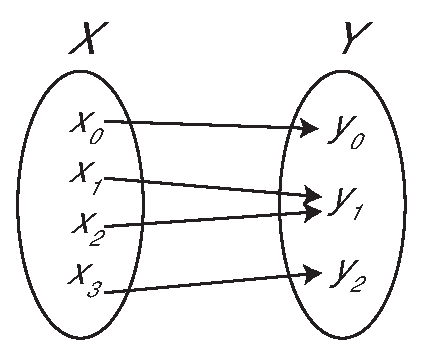
\includegraphics[width=6cm]{img/surjection.eps}
    \caption{Każdemu wejściu przyporządkowywane jest dokładnie jedno wyjście}
    \label{fig:surjection}
\end{figure}

Kryptograficzna funkcja skrótu to taka funkcja skrótu, która może być
wykorzystywana w~zastosowaniach kryptograficznych, a~więc wymagających
wysokiego poziomu bezpieczeństwa. Przykłady takich zastosowań można znaleźć
w~sekcji~\ref{sec:secure_hash_usages}. Dokładne cechy, jakie powinna spełniać
funkcja skrótu, aby była kryptograficzna, omówione zostały w~sekcji
~\ref{sec:secure_hash_attributes}. Ponadto wszystkie funkcje skrótu,
niezależnie od swojego zastosowania w~celach kryptograficznych, powinny
spełniać własności opisane w~sekcji~\ref{sec:common_hash_attributes}.



\subsubsection{Cechy zwykłych funkcji haszujących}
\label{sec:common_hash_attributes}
Niezależnie od swojego zastosowania, każda funkcja haszująca musi spełniać
pewne warunki, które zostały poniżej opisane.

\myparagraph{Determinizm}
Funkcje haszujące powinny być deterministyczne w~takim sensie, że ich wyniki
zależą wyłącznie od danych wejściowych, a~nie żadnych czynników losowych.
Innymi słowy, haszowanie wiadomości $m$ powinno dawać taki sam skrót
niezależnie od okoliczności. Stąd wynika, że funkcje skrótu nie powinny się
nigdy odwoływać do generatorów liczb pseudolosowych, metadanych o~wiadomości
(typu jej lokalizacja w~pamięci komputera) itp., a~jedynie do samej wiadomości.

\myparagraph{Jednostajność}
Niech $H : A \to B$ będzie funkcją haszującą. Funkcje haszujące powinny
przekształcać wartości ze zbioru wejściowego $A$ na wartości ze zbioru
wyjściowego $B$ w~taki sposób, by:
\[
    \forall_{a \in A} \; \Pr(H(a) = b) \to \frac{1}{|B|}
\]
Innymi słowy dobra funkcja haszująca przekształca konkretną wartość $a$
w~konkretną wartość $b$ z~prawdopodobieństwem jak najbliższym
prawdopodobieństwu losowego wybrania tego elementu ze zbioru $B$, lub też~--
dla danej wiadomości $m$ wszystkie wartości ze zbioru $B$ powinny mieć możliwie
taką samą szansę na wybranie (z zachowaniem własności determinizmu). Cecha ta
ma na celu zapewnienie jak najmniejszego prawdopodobieństwa zajścia kolizji.

Unikanie kolizji, obok determinizmu, jest jedną z~najważniejszych cech funkcji
skrótu, co staje się zrozumiałe, gdy pozna się ich zastosowania (przykładowe
zastosowania bezpiecznych funkcji skrótu opisane są
w~sekcji~\ref{sec:secure_hash_usages}).



\subsubsection{Cechy kryptograficznych funkcji haszujących}
\label{sec:secure_hash_attributes}
Aby lepiej zrozumieć naturę warunków nałożonych na cechy kryptograficznych, lub
też \emph{bezpiecznych} funkcji skrótu, należy uświadomić sobie ich naturę:
w~sytuacji, kiedy kolizje są tylko niepożądane, sięgamy po zwykłe funkcje
haszujące, funkcje kryptograficzne stają się natomiast potrzebne wówczas, gdy
kolizje są \emph{niedopuszczalne}.

Jednak z~racji mniejszego rozmiaru przeciwdziedziny w~stosunku do dziedziny
(patrz rysunek~\ref{fig:surjection} na stronie \pageref{fig:surjection}),
kolizje \emph{będą} się zdarzać.

Poniższe warunki zostały sformułowane po to, aby sytuacje, w~których dochodzi
do kolizji, były jak najmniej prawdopodobne i~żeby było trudno je celowo
wywołać, a~także żeby same kryptograficzne funkcje skrótu stanowiły godne
użycia narzędzie we wszystkich sytuacjach, które wymagają wysokiego
bezpieczeństwa.

\myparagraph{Odporność na kolizje pierwszego rzędu (\en{preimage resistance})}
\label{sec:preimage_resistance}
Mając dany skrót $h$, znalezienie wiadomości $m$ takiej, że $H(m) = h$ powinno
być w~praktyce niewykonalne. Jest to warunek zapewniający jednostronność
funkcji skrótu. Należy zauważyć, że zależy nam na \emph{dowolnej} wiadomości,
a~nie oryginalnej wiadomości z~której zostało utworzone $h$.

\myparagraph{Odporność na kolizje drugiego rzędu (\en{second preimage
resistance})}
\label{sec:second_preimage_resistance}
Mając daną wiadomość $m$, znalezienie wiadomości $m' \neq m$ takiej, że $H(m) =
H(m')$ powinno być praktycznie niewykonalne.

\myparagraph{Odporność na kolizje (\en{collision resistance})}
\label{sec:collision_resistance}
Znalezienie dwóch dowolnych różnych wiadomości $m \neq m'$ takich, że $H(m) =
H(m')$ powinno być praktycznie niewykonalne. Spełnienie tej własności implikuje
odporność na kolizje drugiego rzędu, co jednak nie implikuje odporności na
kolizje pierwszego rzędu.

\myparagraph{Niemożność odróżnienia od \en{random oracles}}
\en{Random oracle} to teoretyczna czarna skrzynka przypisująca każdemu
argumentowi losową (z jednostajnym rozkładem prawdopodobieństwa) wartość
z~określonej przeciwdziedziny w~taki sposób, że dla konkretnego argumentu
zawsze wybiera taką samą wartość. Jest to abstrakcyjna funkcja matematyczna,
o~której udowodniono~\cite{random_oracle}, że nie może posiadać żadnej
implementacji. Pożądane jest to, by kryptograficzna funkcja skrótu była trudna
do odróżnienia od \en{random oracle}, choć jest to zadanie znacznie trudniejsze
od spełnienia poprzednich własności.

\myparagraph{Własność efektu lawinowego}
\label{sec:avalance_effect}
W~dobrych funkcjach haszujących powinien zachodzić tzw. efekt lawinowy. Jest to
własność zapewniająca, że nawet mała zmiana wiadomości $m'$ w~stosunku do $m$
powoduje duże zmiany w~wartości $H(m')$ w~porównaniu do $H(m)$. Jej celem jest
zapewnienie jednej z~dwóch fundamentalnych własności dobrego systemu
kryptograficznego, sformułowanych przez Shannona
w~1949~\cite{confusion_diffusion}~-- kryteriów \en{confusion and diffusion}
(zamieszanie i~rozpraszanie). Warunki te mówią o~tym, że zależności pomiędzy
wiadomością a~jej szyfrogramem oraz między szyfrogramem a~kluczem użytym do
szyfrowania powinny być jak najbardziej skomplikowane i~nieprzewidywalne tak,
by utrudnić potencjalne ataki.

\noindent Formalnie mówi się o~dwóch, wymienionych poniżej, kryteriach efektu
lawinowego.

\begin{myenumerate}

    \item Ścisłe kryterium lawinowe (\en{strict avalanche criterion},
    \abbr{SAC}): po zmianie dowolnego bitu wejścia, każdy bit wyjścia powinien
    się zmienić z~prawdopodobieństwem równym $\frac{1}{2}$.

    \item Kryterium niezależności bitowej (\en{bit independence criterion},
    \abbr{BIC}): po zmianie dowolnego bitu wejścia, każde dwa bity wyjścia
    powinny zmieniać się w~sposób niezależny od siebie.

\end{myenumerate}

\begin{figure}[hbt!]
    \pgfplotsset{width=14cm,height=7cm}
    \begin{tikzpicture}
        \newcommand{\tmp}{$\Pr(H(a)_{(2,i)}=1)$}
        \begin{axis}[xlabel=$i$-ty bit,ylabel=\tmp,/pgf/number
        format/.cd,fixed,precision=3]
        \addplot[color=blue,mark=*] coordinates {
            (0, 0.501249577499)
            (1, 0.50207665441)
            (2, 0.500985834708)
            (3, 0.500601743263)
            (4, 0.498658240554)
            (5, 0.499766984524)
            (6, 0.50055309168)
            (7, 0.498996241025)
            (8, 0.50000256061)
            (9, 0.500978152879)
            (10, 0.499813075497)
            (11, 0.500092181947)
            (12, 0.500104984995)
            (13, 0.500038409144)
            (14, 0.499416181004)
            (15, 0.500189485113)
            (16, 0.500914137638)
            (17, 0.499784908791)
            (18, 0.49979515123)
            (19, 0.499108907849)
            (20, 0.499188286747)
            (21, 0.501026804462)
            (22, 0.49944690832)
            (23, 0.501011440804)
            (24, 0.500547970461)
            (25, 0.49958262063)
            (26, 0.49972345416)
            (27, 0.500340561081)
            (28, 0.500975592269)
            (29, 0.498632634458)
            (30, 0.500924380076)
            (31, 0.500058894021)
            (32, 0.499833560374)
            (33, 0.500975592269)
            (34, 0.499229256501)
            (35, 0.500862925445)
            (36, 0.499746499647)
            (37, 0.500788667766)
            (38, 0.499434105272)
            (39, 0.500023045487)
            (40, 0.500842440568)
            (41, 0.498863089324)
            (42, 0.4979259062)
            (43, 0.500245818524)
            (44, 0.499352165764)
            (45, 0.500660637285)
            (46, 0.49937521125)
            (47, 0.499946227198)
            (48, 0.499559575144)
            (49, 0.500455788514)
            (50, 0.500325197423)
            (51, 0.499492999293)
            (52, 0.499490438684)
            (53, 0.499341923325)
            (54, 0.500399455102)
            (55, 0.50075794045)
            (56, 0.499221574672)
            (57, 0.500535167413)
            (58, 0.500862925445)
            (59, 0.499869408909)
            (60, 0.501812911618)
            (61, 0.501142031895)
            (62, 0.500194606332)
            (63, 0.501666956869)
            (64, 0.501326395788)
            (65, 0.499114029068)
            (66, 0.498932225784)
            (67, 0.49992830293)
            (68, 0.499149877603)
            (69, 0.499718332941)
            (70, 0.500181803284)
            (71, 0.49868384665)
            (72, 0.498258785452)
            (73, 0.501003758975)
            (74, 0.499784908791)
            (75, 0.499211332234)
            (76, 0.499664560138)
            (77, 0.501646471992)
            (78, 0.49889381664)
            (79, 0.500637591798)
            (80, 0.499536529657)
            (81, 0.499526287218)
            (82, 0.499500681122)
            (83, 0.5010370469)
            (84, 0.500299591327)
            (85, 0.4996543177)
            (86, 0.499969272684)
            (87, 0.498530210072)
            (88, 0.499974393904)
            (89, 0.499528847828)
            (90, 0.500094742556)
            (91, 0.500094742556)
            (92, 0.499769545133)
            (93, 0.500737455573)
            (94, 0.500875728493)
            (95, 0.500722091916)
            (96, 0.500542849242)
            (97, 0.499431544662)
            (98, 0.500778425328)
            (99, 0.499244620159)
            (100, 0.499989757561)
            (101, 0.498786271035)
            (102, 0.500578697776)
            (103, 0.500169000236)
            (104, 0.499841242203)
            (105, 0.50027398523)
            (106, 0.500156197187)
            (107, 0.500640152407)
            (108, 0.499116589678)
            (109, 0.500645273627)
            (110, 0.500099863776)
            (111, 0.49951348417)
            (112, 0.499918060492)
            (113, 0.500512121926)
            (114, 0.49979515123)
            (115, 0.499669681358)
            (116, 0.500225333647)
            (117, 0.501841078324)
            (118, 0.499879651347)
            (119, 0.498970634929)
            (120, 0.500312394375)
            (121, 0.50041481876)
            (122, 0.499160120041)
            (123, 0.499188286747)
            (124, 0.49889381664)
            (125, 0.500145954749)
            (126, 0.499733696598)
            (127, 0.500734894964)
        };
        \end{axis}
    \end{tikzpicture}
    \caption{Przykładowy rozkład prawdopodobieństwa występowania ``1'' na
    kolejnych bitach skrótów \texttt{MD5}, otrzymanych z~zahaszowania wyrazów
    z~listy~\ref{wl:english_wordlist} w~dodatku~\ref{app:wordlists}.}
    %todo: wspomnieć o programie z dodatku C
    \end{figure}
\pagebreak



\subsection{Zastosowania kryptograficznych funkcji skrótu}
\label{sec:secure_hash_usages}
Same funkcje skrótu mają bardzo szerokie zastosowania, my jednak skupimy się
wyłącznie na zastosowaniach \emph{kryptograficznych} funkcji haszujących.
W~każdym przypadku opisane zastosowanie utylizuje podstawową cechę
kryptograficznych funkcji skrótu, jaką jest odporność na kolizje.



\subsubsection{Weryfikacja integralności danych}
\label{sec:usage_integrity_check}
Wyobraźmy sobie sytuację, w~której użytkownik o~imieniu Alicja zmuszony jest
przetransportować jakieś dane przez niebezpieczny kanał informacji, który jest
podatny na zakłócenia, do użytkownika imieniem Bob. Niech wiadomość wysłana
przez Alicję oznaczona będzie $m$, a~wiadomość odebrana przez Boba będzie $m'$.

\begin{figure}[htb!]
    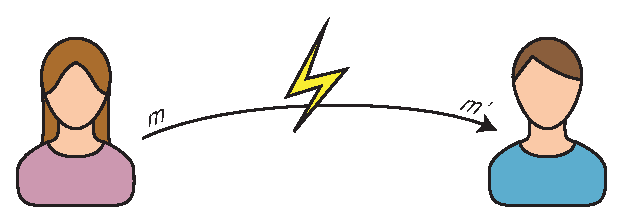
\includegraphics[width=10cm]{img/usage1.eps}
    \caption{Wiadomość odebrana przez Boba niekoniecznie musi dotrzeć do niego
    w~formie identycznej jak podczas nadania przez Alicję}
    \label{fig:usage_integrity_check_1}
\end{figure}

Z~taką transmisją wiąże się wiele problemów, gdy zaczniemy rozpatrywać ją pod
kątem zapewnienia bezpieczeństwa. Jednym z~takim problemów jest zapewnienie
bezpiecznego mechanizmu weryfikacji, czy dane odebrane przez Boba są faktycznie
tymi samymi danymi, które były wysłane do niego przez Alicję, a~więc czy nie
zostały zmienione w~jakikolwiek sposób podczas transportu. Innymi słowy, należy
w~jakiś sposób zweryfikować, czy $m' = m$.

Z~pomocą w~rozwiązaniu tego problemu przychodzą funkcje haszujące. Alicja może,
obok samej wiadomości $m$, przesłać wyliczony u~siebie skrót tej wiadomości,
$h=H(m)$. Bob może wówczas zweryfikować integralność odebranych danych $m'$
poprzez obliczenie ich skrótu po swojej stronie $H(m')=h'$, a~w~następnej
kolejności porównanie samych skrótów (sprawdzenie, czy obliczony przez Alicję
$h$ jest równy obliczonemu przez niego $h'$).

\begin{figure}[htb!]
    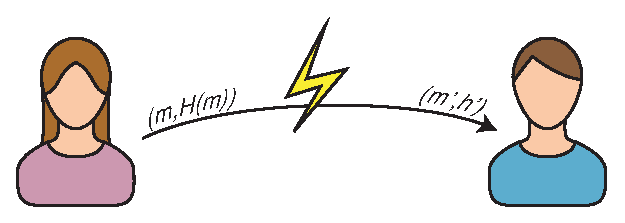
\includegraphics[width=10cm]{img/usage1b.eps}
    \caption{Bob ma teraz dodatkowy mechanizm weryfikacji integralności~--
    wystarczy, że sprawdzi, czy $H(m')=h'$.}
    \label{fig:usage_integrity_check_2}
\end{figure}

Wprowadzenie funkcji haszujących właśnie pozwoliło sprowadzić problem
zabezpieczenia transmisji potencjalnie bardzo długich komunikatów do
zabezpieczenia transmisji jedynie samych skrótów.

Należy zdawać sobie sprawę, że nie rozwiązuje to problemu zabezpieczenia
transmisji przed rozmyślnymi atakami~-- jeśli ktoś mógł wcześniej zmieniać
zawartość $m$, teraz może również zmienić wartość $h$ zawierającą $H(m)$.
Ponadto funkcje haszujące nie zapewniają żadnej poufności danych. Mimo to z~ich
zastosowania płyną pewne wymienione niżej korzyści.

\begin{itemize}

    \item Rozwiązanie to jest przydatne w~sytuacjach, kiedy nie mamy do
    czynienia z~rozmyślnymi atakami, a~jedynie przypadkowymi zakłóceniami~--
    prawdopodobieństwo, że skrót $H(m')$ będzie równy $H(m)$ w~sytuacji, kiedy
    $m \neq m'$ będzie minimalne. Jest to jedno z~naturalnych zastosowań
    funkcji haszujących, w~których odgrywają rolę trudnej do podrobienia sumy
    kontrolnej.

    \item Ponadto ułatwione jest tworzenie innych protokołów~-- dzięki funkcjom
    haszującym zależy nam na zabezpieczeniu przed modyfikacją nie całej
    wiadomości, a~jedynie jej malutkiego kawałka zawierającego skrót.
    Przykładem protokołu, który pracuje na opisanej powyżej zasadzie, jest
    podpis elektroniczny~-- \latin{de~facto} weryfikuje się tam wyłącznie
    autentyczność skrótu wiadomości, a~nie samą wiadomość.

\end{itemize}



\subsubsection{Bezpieczne przechowywanie / weryfikacja haseł}
\label{sec:usage_password_check}
Funkcje haszujące przychodzą z~pomocą także w~technikach przechowywania haseł.
Wyobraźmy sobie przeciętny mechanizm autentykacji.

\begin{myenumerate}

    \item Użytkownik Alicja przesyła swoje dane uwierzytelniające do serwera.

    \item Serwer odbiera dane $m$.

    \item Serwer porównuje dane $m$ z~wzorcem $m'$ przechowywanym w~bazie
    danych: \label{enu:server_pass_check}

    \begin{myenumerate}

        \item jeżeli dane się zgadzają ($m = m'$), serwer udziela Alicji
        dostępu,

        \item w~przeciwnym wypadku odmawia dostępu.

    \end{myenumerate}

\end{myenumerate}

Z~takim podejściem wiążą się pewne problemy. Po pierwsze, dane, która przesyła
Alicja, mogą zostać przechwycone przez osobę trzecią, zatem wymagają
zaszyfrowania (np. poprzez zaszyfrowanie transmisji protokołem \texttt{HTTPS}).
Jednak nie ten problem okazuje się ważny z~punktu widzenia funkcji haszujących.
Nas zainteresuje problem wiążący się z~punktem~\ref{enu:server_pass_check}~--
co w~wypadku, kiedy do bazy danych serwera, z~jakichkolwiek przyczyn, uzyskuje
dostęp ktoś niepożądany? Taka osoba może wówczas podejrzeć dane
uwierzytelniające \emph{wszystkich} użytkowników, także Alicji, a~następnie
pomyślnie zalogować się przy pomocy tak wykradzionych danych.

Musimy zatem jakoś zabezpieczyć bazę danych. Można próbować ją szyfrować lub
inaczej zabezpieczać dane w~niej przechowywane, problem z~takim podejściem jest
jednak taki, że na pewnym poziomie tak czy inaczej jakaś osoba (administrator)
zawsze będzie miał dostęp do fizycznych danych. Możemy także zahaszować dane
uwierzytelniające i~zmodyfikować nasz protokół w~sposób opisany poniżej.

\begin{myenumerate}

    \item Użytkownik Alicja przesyła swoje dane uwierzytelniające do serwera.

    \item Serwer odbiera dane $m$.

    \item Serwer wylicza na ich podstawie hasz $h = H(m)$.

    \item Serwer porównuje hasz $h$ z~wzorcowym haszem $h'$ przechowywanym
    w~bazie danych:

    \begin{myenumerate}

        \item jeżeli skróty się zgadzają ($h = h'$), serwer udziela Alicji
        dostępu,

        \item w~przeciwnym wypadku odmawia dostępu.

    \end{myenumerate}

\end{myenumerate}

Dzięki temu, że w~bazie przechowywane są jedynie nieodwracalne skróty, nawet
w~przypadku kradzieży bazy danych na podstawie wykradzionych skrótów nie
powinno być można odtworzyć oryginalnych danych (patrz
punkt~\ref{sec:preimage_resistance}). Teoretycznie zatem atakującemu taka baza
w~zasadzie do niczego się nie przyda.

Należy jednak zwrócić uwagę, że protokół ten nie jest bezpieczny bez pewnych
poprawek. Przyczyny i~natura poprawek omówione są
w~części~\ref{sec:universal_attacks}.



\subsubsection{Jednoznaczna identyfikacja danych}
Innym zastosowaniem funkcji haszujących jest identyfikacja ciągów bajtów,
a~w~szerszym ujęciu~-- plików, struktur/obiektów programistycznych itp. Poniżej
znajdują się przykłady wykorzystania tego pomysłu w~różnego rodzaju
rozwiązaniach.

\begin{itemize}

    \item Systemy kontroli wersji, w~tym Mercurial oraz Git, wykorzystują
    funkcje skrótu w~celu bezpiecznej identyfikacji konkretnych wersji pliku,
    numerowania kolejnych zmian i~bezpiecznego przechowywania historycznej
    struktury repozytorium.

    \item Linki ed2k oraz magnet, używane w~sieciach peer-to-peer, wykorzystują
    funkcje skrótu w~celu lokalizacji źródeł, skąd dany plik może być pobrany,
    a~także weryfikacji już ściągniętych danych (patrz
    punkt~\ref{sec:usage_integrity_check}).

    \item Struktury danych takie jak tablice mieszające (tzn. tablice, których
    kluczami może być dowolny obiekt, w~przeciwieństwie do klasycznych tablic
    o~indeksach liczbowych), wykorzystują funkcje haszujące do serializacji
    dowolnych obiektów na taką postać, jaką ich algorytmy indeksowania są
    w~stanie obsłużyć. Przykładowo, w~języku Java każdy zdefiniowany przez
    użytkownika obiekt powinien zaimplementować metodę \texttt{hashCode()},
    która w~zamierzeniu ma pozwolić łatwo odróżniać (na~tyle, na~ile to
    możliwe) konkretne instancje obiektu w~stosunku do pozostałych.

\end{itemize}

\begin{figure}[bht]
    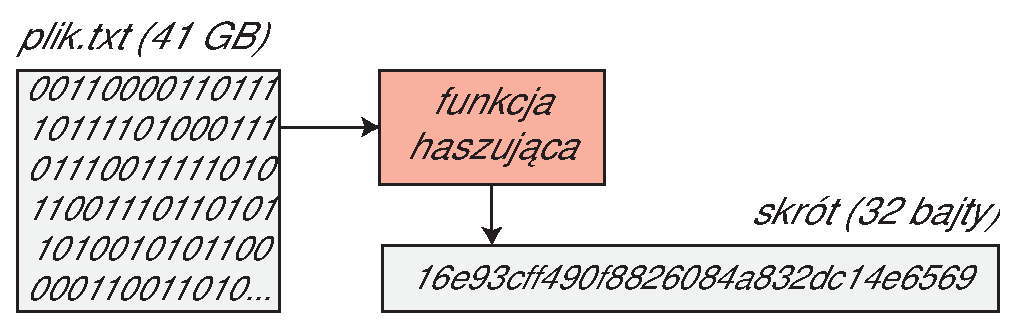
\includegraphics[width=12cm]{img/usage3.eps}
    \caption{Gdy trzeba zweryfikować poprawność przesłania dużej struktury,
    łatwiej porównać krótki skrót}
\end{figure}

Biorąc pod uwagę fakt, że kryptograficzne funkcje skrótu są dużo bardziej
kosztowne obliczeniowo niż zwykłe, nieodporne na ataki funkcje haszujące,
w~większości tego typu zastosowań korzystanie z~kryptograficznych funkcje
skrótu postrzegane jest jako przesada i~stosowane są zwyczajne funkcje skrótu.
Mimo to, czasem jednak bezpieczeństwo jest konieczne, szczególnie w~sytuacjach
opisanych powyżej, gdzie ryzyko ataku jest wysokie. Przykładowo, atakujący może
stworzyć plik zawierający wirus, którego hasz byłby taki sam jak skrót całkiem
niewinnego pliku, po czym umieścić taki plik w~sieci peer-to-peer~-- dzięki
zastosowaniu kryptograficznych funkcji skrótu, taki scenariusz jest bez
porównania trudniejszy do skutecznego przeprowadzenia.



\subsection{Rys historyczny}
Historia funkcji haszujących sięga późnych lat 70--tych. W~roku 1976 Diffie
i~Hellman w~swojej pracy traktującej o~kryptografii z~kluczem publicznym,
opisali zapotrzebowanie na funkcję mapującą ciągi bitów dowolnej długości na
ciągi bitów ograniczonej długości w~nieodwracalny sposób. W~roku 1978 Rabin po
raz pierwszy zaproponował funkcję skrótu opartą na 64--bitowym wariancie
blokowego algorytmu szyfrującego DES. W~1979 roku Yuval opisał sposób, jak
wykorzystując paradoks urodzinowy złamać $n$--bitową funkcję haszującą w~czasie
$2^{n/2}$.

W~tym samym roku zaczęły się pojawiać pierwsze próby zdefiniowania warunków,
jakie powinny spełniać bezpieczne funkcje skrótu. W~1979 Merkle wprowadził
pojęcie odporności na kolizje oraz odporności pierwszego i~drugiego rzędu
(patrz sekcja~\ref{sec:secure_hash_attributes}). Definicje te zostały
ostatecznie sformalizowane przez Damg\r{a}rda w~roku 1987. W~roku 2004 Rogaway
i~Shrimpton pokazali, że funkcje haszujące w~miarę możliwości nie powinny być
odróżnialne od \en{random oracles}.

Już od samego początku, czyli późnych lat 70--tych, funkcje haszujące
przeżywały bardzo szybki rozwój. Zapotrzebowanie na bezpieczne i~szybkie
funkcje skrótu było szeroko rozumiane, nie zaskakuje zatem fakt, że do lat
90--tych znane było już około 50 konstrukcji. Pierwsi kandydaci korzystali
z~dorobku blokowych funkcji szyfrujących; w~późniejszym okresie rozwoju
niektórzy poszli w~kierunku teoretycznych konstrukcji opartych na algebrze
liniowej. Z~czasem jednak zaniechano adaptowania mechanizmów sprawdzonych
w~innych zastosowaniach na rzecz tworzenia dedykowanych funkcji.

Tak naprawdę do dnia dzisiejszego niewiele się zmieniło: od lat mamy do
czynienia z~ciągłym procesem wykazywania słabości istniejących rozwiązań
i~w~odpowiedzi wymyślania kolejnych usprawnień bądź całkiem nowych konstrukcji.
Proces ten zyskał nawet niedawno własne wydarzenie medialne w~postaci konkursu
ogłoszonego przez \enn{National Institute of Standards and Technology}, mającego
na celu wyłonienie następcy funkcji haszujących \texttt{SHA-1} i~\texttt{SHA-2}
spośród kilkudziesięciu kandydatów zgłoszonych przez kryptologów z~całego
świata. Cykl ten będzie prawdopodobnie trwał tak długo, aż zostanie odkryta
uniwersalna nieodwracalna funkcja skrótu lub wykazana zostanie niemożność
stworzenia takowej.



\section{Konstrukcja funkcji haszujących}
\label{sec:hash_construction}
Wprawdzie konstrukcji funkcji haszujących jest wiele, większość z~nich wygląda
podobnie. Na początku skupię się na teoretycznych aspektach konstruowania
funkcji haszujących, a~w~następnej kolejności opiszę praktyczne implementacje.



\subsection{Doskonała funkcja skrótu}
W~teorii mówi się o~doskonałej funkcji skrótu, która każdy element $m$ z~danego
zbioru $M$ potrafi przekształcić w~sposób bezkolizyjny w~$h$ z~tego samego
zbioru. Innymi słowy, jest to bijekcja na samą siebie, lub permutacja.

\begin{figure}[htb!]
    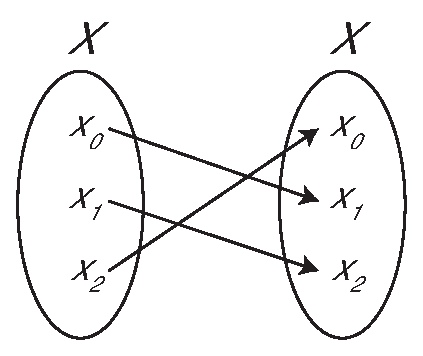
\includegraphics[width=6cm]{img/injection_self.eps}
    \caption{Każdemu wyjściu przyporządkowywane jest dokładnie jedno wejście}
    \label{fig:bijection}
\end{figure}


Znalezienie takiej funkcji w~praktyce polega na użyciu algorytmu losowego,
który dobiera każdemu $m$ przypadkowy element $h$ tak długo, aż $h$ będzie
niewykorzystany przez żaden inny element (czyli zapewniony będzie brak
kolizji):

\begin{myenumerate}

    \item Zainicjuj tablicę podstawień $T$

    \item Dla każdego $m \in M$:

    \begin{myenumerate}

        \item Wylosuj $h \in M$ takie, że $\not \exists_{m' \in M} : T_{m'} =
        h$

        \item Przydziel $T_m = h$

    \end{myenumerate}

\end{myenumerate}

Taka funkcja, mimo że na pierwszy rzut oka wydaje się przydatna
w~zastosowaniach kryptograficznych (jak by nie patrzeć, implementuje całkowicie
losowe permutacje!), jest podejściem złym z~prostych przyczyn:

\begin{itemize}

    \item Algorytm przekształcania elementów $m \in M$ na $h$ polega na
    trywialnym podstawianiu elementów zgodnie z~jakąś tablicą $T$. Zatem, aby
    uzyskać oryginalne $m$ na podstawie $h$ wystarczy odwrócić tablicę,
    zamieniając jej klucze z~przypisanymi im wartościami (dla danego $h$
    wyszukać $m$, dla którego $T_m = h$). Wykazaliśmy w~ten sposób brak
    własności \en{preimage resistance}.

    \item Gdy natomiast będziemy próbowali ukryć sposób w~jaki dokonujemy
    podstawienia (innymi słowy utajnić tablicę $T$), mamy do czynienia
    z~\en{security through obscurity} (bezpieczeństwo poprzez niezrozumiałość),
    co jest bardzo negatywnym zjawiskiem w~kryptografii i~łamie tzw. zasadę
    Kerckhoffsa. Zasada ta jest jedną z~kilku reguł sformułowanych w~XIX w.
    przez Kerckhoffsa, traktujących na temat bezpieczeństwa kryptosystemów.
    Mówi ona, że każdy system kryptograficzny musi być bezpieczny nawet, gdy
    jego sposób działania wraz ze szczegółami implementacji jest jawny (za
    wyjątkiem klucza, który jest z~definicji tajny, z~tym że funkcje haszujące
    nie używają klucza).

    \item Nawet gdy zignorujemy powyższe przykazanie, nasz algorytm będzie
    nieodporny na proste ataki statystyczne: analizując rozkład
    prawdopodobieństwa pewnych wzorców wewnątrz kolejnych $h$ (który nie jest
    jednostajny, jako że w~praktyce rzadko kiedy wejście ma rozkład
    jednostajny), możemy zyskać ogólne wyobrażenie o~tym, jak wyglądają wzorce
    wewnątrz $m \in M$, co może nas doprowadzić do oryginalnych $m$.

    \item Wreszcie, funkcja taka jest bardzo niepraktyczna: po pierwsze, musimy
    znać z~góry \emph{wszystkie} możliwe wiadomości, jakie możemy chcieć
    zahaszować; mało tego~-- wiadomości te muszą mieć tę samą długość. Powoduje
    to, że funkcja ta nie nadaje się na kryptograficzną funkcję skrótu.

\end{itemize}



\subsection{Funkcja jednokierunkowa}
Funkcja jednokierunkowa to funkcja, której wartości dla każdego wejścia da się
łatwo obliczyć; powinno być trudne natomiast obliczenie wejścia na podstawie
posiadanego konkretnego wyjścia.

\noindent Nieformalnie, funkcja $f$ jest silnie jednokierunkowa, jeśli:

\begin{itemize}

    \item da się obliczyć w~czasie wielomianowym (czyli w~taki sposób, że czas
    działania $f$ jest w~sposób wielomianowy zależny od rozmiaru danych
    wejściowych),

    \item żaden probabilistyczny algorytm działający w~czasie wielomianowym nie
    potrafi zgadnąć argumentu z~zaniedbywalnie małym
    prawdopodobieństwem~\cite{one_way_functions}.

\end{itemize}

\noindent $f$ jest natomiast słabo jednokierunkowa, jeśli:

\begin{itemize}

    \item da się obliczyć w~czasie wielomianowym,

    \item każdy probabilistyczny algorytm działający w~czasie wielomianowym,
    który ją potrafi odwrócić, zgaduje argumenty w~sposób niepoprawny
    z~niezaniedbywalnie dużym prawdopodobieństwem~\cite{one_way_functions}.

\end{itemize}

Łatwo zauważyć, że każda silnie jednokierunkowa funkcja spełnia jednocześnie
warunki nałożone na funkcje słabo jednokierunkowe. Ponadto każda funkcja
jednokierunkowa spełnia automatycznie podstawowy warunek nałożony na bezpieczne
funkcje skrótu (mianowicie \en{preimage collision resistance}). Funkcje te
powinny zatem przyciągnąć nasze zainteresowanie.



\subsubsection{$\textrm{P} \neq \textrm{NP}$?}
Problem z~funkcjami jednokierunkowymi jest niestety taki, że\ldots nie
udowodniono~\cite{one_way_functions_existence} ich istnienia. Istnieją pewne
funkcje, które podejrzewamy o~jednokierunkowość, lecz nie potrafimy wykazać
poprawności lub niepoprawności tego podejrzenia.
Wykazano~\cite{one_way_functions}, że z~istnienia słabo jednokierunkowych
funkcji wynika istnienie silnie jednokierunkowych funkcji. Ponadto
udowodniono~\cite{one_way_functions}, że istnienie funkcji jednokierunkowych
implikowałoby jednocześnie, że $\textrm{P} \neq \textrm{NP}$, co dałoby
odpowiedź na jeden z~problemów milenijnych i~oznaczałoby, że klasa problemów,
które da się \emph{rozwiązać} w~czasie wielomianowym ($\textrm{P}$) nie pokrywa
się z~klasą, dla którego rozwiązanie da się \emph{zweryfikować} w~czasie
wielomianowym ($\textrm{NP}$). Przykładowo: mając liczbę $x \in \mathbb{N}$
i~dany zbiór liczb pierwszych $x_i$, możemy w~banalny sposób
\emph{zweryfikować}, czy $x_0 \cdot x_1 \cdot \ldots \cdot x_n = x$. Natomiast
nie wiadomo, czy istnieje algorytm wielomianowy, który potrafi \emph{rozwiązać}
ten problem, znajdując dla danego $x$ liczby pierwsze $x_0, x_1, \ldots, x_n$
takie, że $x_0 \cdot x_1 \cdot \ldots \cdot x_n = x$. Problem ten jest znany
jako problem rozkładu liczby na czynniki pierwsze, lub inaczej problem
faktoryzacji, i~stanowi pierwszy ze wspominanych kandydatów na funkcje
jednokierunkowe.



\subsubsection{Problem faktoryzacji}
Niech $f(S) = \prod_{s \in S} s$, gdzie $S$ jest dowolnym zbiorem liczb
pierwszych oraz $x \in \mathbb{N}$. Obliczenie $f(S)$ jest trywialne. Natomiast
obliczenie wartości odwróconej funkcji $f^{-1}(x)=S$, a~więc znalezienie dla
danej liczby $x$ jej czynników pierwszych, jest trudne, tzn. nieznany jest
żaden algorytm, który by to potrafił realizować w~czasie zależnym wielomianowo
od rozmiaru $x$.



\subsubsection{Problem logarytmu dyskretnego}
Niech $f(x, p, g) = g^x \mod p$, gdzie $p$ jest liczbą pierwszą, $g < p$ oraz
$x < p$. Wyliczenie tej wartości jest trywialne; nie znamy natomiast algorytmu
wielomianowego pozwalającego na zgadnięcie wartości odwróconej funkcji
\mbox{$f^{-1}(y, p, g) = x : g^x \mod p = y$} na podstawie danego $y$. Nazwa
problemu wynika z~charakteru $f$ (operacją odwrotną do potęgowania w~ciele
modulo $p$ jest logarytm w~ciele modulo $p$).



\subsubsection{Funkcja Rabina}
Niech $f(x,n) = x^2 \mod n$. Wykazano, że obliczenie $f^{-1}(y,n) = x : x^2
\mod n = y$ na podstawie $y$ i~$n$ jest tak samo trudne, jak rozkład $n$ na
czynniki pierwsze; co sprowadza się do problemu faktoryzacji, opisanego
wcześniej.



\subsubsection{Wnioski}
Zastosowania funkcji jednokierunkowych są niejako podzbiorem tego, do czego
potrzebujemy bezpiecznych funkcji haszujących: łatwe obliczenie $f(x)$, łatwa
weryfikacja $f(x)=f(x')$ i~trudne uzyskanie odwróconej funkcji $f^{-1}(y)=x$.
Stąd też nie powinno dziwić, że ostatnim, niewspomnianym dotąd kandydatem na
funkcje jednokierunkowe są\ldots kryptograficzne funkcje skrótu.

Zapotrzebowanie na funkcje jednokierunkowe jest duże, o~czym świadczy ich
wykorzystanie: trudność faktoryzacji jest zastosowana w~kryptosystemie RSA,
trudność obliczenia logarytmu dyskretnego w~podpisach cyfrowych ElGamala,
a~trudność obliczenia pierwiastka dyskretnego (funkcja Rabina)~--
w~kryptosystemie Rabina. Trudność złamania tych kryptosystemów opiera się
właśnie na trudności odwrócenia wymienionych funkcji.

Wracając na chwilę do zagadnienia $\textrm{P} \stackrel{?}{=} \textrm{NP}$~--
wystarczy udowodnić, że którakolwiek z~powyższych funkcji jest faktycznie
jednokierunkowa lub pokazać, że może zostać złamana, by móc stwierdzić to samo
o~wszystkich pozostałych wymienionych funkcjach. Jest tak dlatego, ponieważ
istnieją sposoby przekształcania jednego problemu w~drugi tak, że rozwiązanie
jednego gwarantuje rozwiązanie drugiego. Zatem tak naprawdę bezpieczeństwo
powyższych kryptosystemów jest do pewnego stopnia równoważne (na tyle, na ile
kosztowne są przekształcenia problemów).



\pagebreak
\subsection{Formalnie bezpieczne funkcje skrótu}
Implementacje funkcji skrótu dzielą się na dwie kategorie. Pierwsza z~nich,
omówiona tutaj, wywodzi się z~formalnego spojrzenia na problem haszowania. Tak
naprawdę metoda ta sprowadza się do wykorzystania opisanych wcześniej
kandydatów na funkcje jednokierunkowe i~dostarczeniu dowodu, że złamanie
konstrukcji opartej na danym problemie jest tak samo trudne, jak trudne jest
rozwiązanie tego problemu. Z~charakteru tego podejścia wywodzi się nazwa tej
rodziny kryptograficznych funkcji haszujących: \en{provably secure
cryptographic hash functions}.

W~praktyce dowody trudności złamania funkcji z~tej rodziny polegają na
pokazaniu istnienia algorytmu, który przekształca w~czasie wielomianowym
problem znajdowania kolizji dla takiej funkcji w~problem rozwiązania źródłowego
problemu. W~ten sposób, kiedy zostanie znaleziony algorytm wielomianowy
potrafiący złamać formalną funkcję haszującą, będzie od razu znany sposób
szybkiego rozwiązywania problemu, na którym ta funkcja się opiera~-- a~na
chwilę obecną zakłada się, że problemy te (faktoryzacja, znajdywanie logarytmu
dyskretnego itp.) są nierozwiązywalne w~czasie wielomianowym, tak więc oznacza
to (najprawdopodobniej) sprzeczność. Możemy zatem powiedzieć, że trudność
złamania formalnych funkcji skrótu jest nie mniejsza niż trudność rozwiązania
dowolnego problemu, o~którym podejrzewamy, że jest trudny do rozwiązania.
Innymi słowy, problem złamania takich funkcji jest redukowalny do problemu
milenijnego, stąd funkcje te są postrzegane jako najbezpieczniejsze dostępne
warianty.



\subsection{Współczesne implementacje}
Wprawdzie formalnie bezpieczne funkcje skrótu są bardzo bezpieczne, nie
przychodzi to bez kosztów. Praktyka pokazuje, że funkcje te prawie w~ogóle się
nie nadają do zastosowań praktycznych lub przemysłowych z~racji swojego wolnego
działania lub wysokich kosztów pamięciowych; niestety, skutecznie eliminuje to
ich przydatność wszędzie tam, gdzie mamy do czynienia z~ograniczonymi zasobami
(przykładami mogą być: systemy wbudowane, transmisje danych w~czasie
rzeczywistym czy też systemy uwierzytelniania o~dużej przepustowości).

W~związku z~tym została stworzona druga rodzina kryptograficznych funkcji
skrótu. Działanie funkcji z~tej rodziny polega ogólnie rzecz biorąc na
dokonywaniu ogromnych ilości różnorodnych operacji na konkretnych bitach
wiadomości $m$ (takich jak przestawianie, dodawanie, odejmowanie i~inne).
Komputery są przystosowane do tego typu obliczeń, dzięki czemu w~porównaniu do
formalnie bezpiecznych funkcji skrótu haszowanie takimi funkcjami odbywa się
bardzo szybko. Oznacza to jednak, że autorzy funkcji zazwyczaj ograniczają się
jedynie do wstępnej analizy jej słabości, \latin{de~facto} nie przedstawiając
formalnego dowodu trudności jej złamania. Badania mające na celu znalezienie
słabości przypominają w~swojej naturze szukanie igły w~stogu siana:
nieznalezienie igły na daną chwilę nie oznacza jeszcze nieistnienia igły. Daje
to pole do popisu kryptologom, którzy znajdują luki na długo po tym, jak dana
funkcja została opisana po raz pierwszy.



\subsubsection{Konstrukcja Merkle-Damg\r{a}rda}
Przykładem sposobu, w~jaki działają nowoczesne kryptograficzne funkcje skrótu
oparte o~operacje bitowe, może być konstrukcja Merkle-Damg\r{a}rda. Opisana po
raz pierwszy przez Merkle w~roku 1979 w~jego pracy
doktorskiej~\cite{merkle_damgard_construction}, stanowi rdzeń używanych po dziś
dzień funkcji skrótu takich jak \texttt{SHA-1} czy \texttt{MD5} i~jest jedną
z~najpopularniejszych metod konstrukcji funkcji haszujących. Konstrukcja ta nie
specyfikuje kompletnego działania~-- wyszczególnione są w~niej natomiast
wymienialne elementy, które muszą być zapewnione przez każdą konkretną
implementację; spośród nich na szczególną uwagę zasługuje funkcja dopełnienia
bitowego oraz funkcja kompresji.

Nazwa wywodzi się stąd, że Merkle oraz Damg\r{a}rd, niezależnie od siebie,
udowodnili~\cite{merkle_damgard_security1,merkle_damgard_security2} w~tym samym
okresie czasu ważną własność tej konstrukcji~-- jeżeli użyty zostanie
odpowiedni schemat dopełnienia bitowego oraz zastosowana funkcja kompresji
będzie odporna na kolizje, to funkcja haszująca zbudowana za pomocą takiej
konstrukcji także będzie odporna na kolizje.

Sama konstrukcja składa się z~kroków opisanych poniżej.

\begin{myenumerate}

    \item Niech $M = \mathtt{Pad}(m)$, gdzie $m$ to wiadomość, a~$\mathtt{Pad}$
    to funkcja dopełnienia bitowego. Zadaniem tej funkcji jest przekształcenie
    wiadomości $m$ o~dowolnej liczbie bitów na wiadomość $M$ o~liczbie bitów
    podzielnej przez z~góry określoną wartość $c$. Trywialnym przykładem
    funkcji dopełnienia bitowego może być funkcja, która dopisuje zera z~prawej
    strony wiadomości $m$.

    \item Podziel $M$ na $n$ bloków, każdy o~stałej długości $c$, niezależnej
    od $m$. Robimy to, ponieważ funkcja kompresji, opisana w~następnych
    krokach, z~definicji może działać jedynie na blokach o~stałej długości $c$.

    \item Niech $h = \mathtt{IV}$, gdzie $\mathtt{IV}$ jest z~góry określonym
    wektorem początkowym (\en{initialization vector}), zawierającą jakaś stałą
    wartość. $h$ będzie się zmieniało wraz z~działaniem konstrukcji i~oznaczać
    będzie aktualnie obliczoną wartość skrótu. Długość $h$ jest przez cały czas
    stała.

    \item Dla $i = 0, 1, \ldots, n$:

    \begin{myenumerate}

        \item Niech $h=\mathtt{Comp}(h,M_i)$, gdzie $\mathtt{Comp}$ jest
        funkcją kompresji, $h$ aktualnie obliczoną wartość skrótu a~$M_i$
        stanowi $i$-ty blok wiadomości $M$.

    \end{myenumerate}

    \item Niech $h=\mathtt{Fin}(h)$ gdzie $\mathtt{Fin}$ jest funkcją
    finalizującą. Jest to opcjonalny krok, który ma zagwarantować dodatkowe
    bezpieczeństwo poprzez np. zapewnienie lepszego efektu lawinowego.

\end{myenumerate}

\begin{figure}[H]
    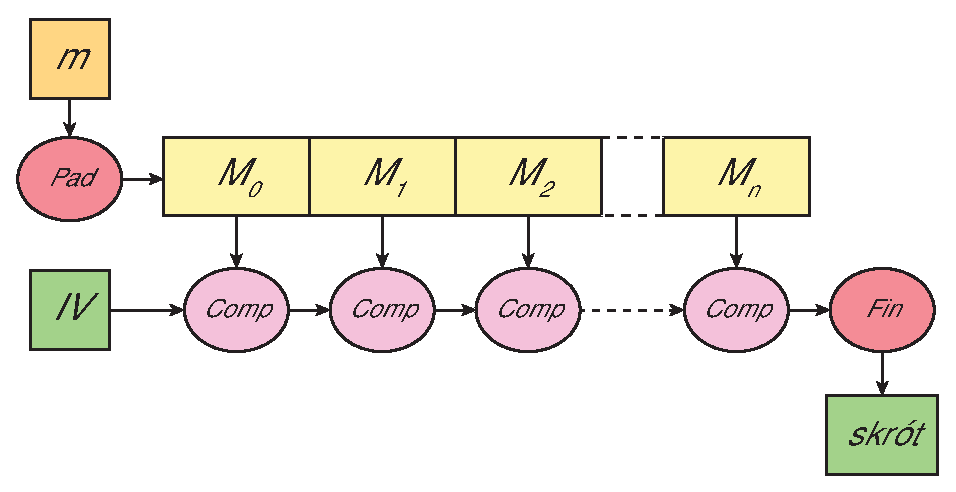
\includegraphics[width=12cm]{img/merkle_damgard.eps}
    \caption{Schemat działania konstrukcji Merkle-Damg\r{a}rda. Oznaczenia:
    $m$~-- wiadomość wejściowa, $\mathtt{Pad}$~-- funkcja dopełnienia bitowego,
    $M_0, M_1, M_2, \ldots, M_n$~-- kolejne bloki wiadomości długości $c$,
    $\mathtt{IV}$~-- wektor początkowy, $\mathtt{Comp}$~-- funkcja kompresji,
    $\mathtt{Fin}$~-- funkcja finalizująca.}
    \label{fig:merkle_damgard}
\end{figure}



\subsubsection{\texttt{MD5}}
\texttt{MD5} jest pierwszą z~dwóch funkcji, na których się skupimy w~tej pracy.
Jej wykorzystanie jest bardzo szerokie; znajduje zastosowanie w~systemach
bezpieczeństwa oraz systemach weryfikacji integralności danych.

Oparta o~konstrukcję Merkle-Damg\r{a}rda, funkcja przekształca wiadomości
o~dowolnej ilości bitów na skróty o~stałej długości 128~bitów. Jej
schemat~\cite{md5_definition} został przedstawiony poniżej (wszystkie operacje
są dokonywane w~porządku bitowym \en{little endian}; znaczenie operatorów
wprowadzonych w~tej sekcji zostało opisane
w~dodatku~\ref{app:bitwise_operations}.

\begin{myenumerate}

    \item Faza dopełnienia bitowego

    \begin{myenumerate}

        \item Dopisz bit $1$ na końcu wiadomości $m$.

        \item Dopisz tyle bitów $0$ na końcu wiadomości $m$, ile potrzeba, aby
        długość $m$ była mniejsza o~64~bity od wielokrotności 512. Innymi
        słowy, dopisz $512 \cdot \ceil{\frac{|m|+64}{512}}-64-(|m| \mod{512})$
        bitów $0$, gdzie $|m|$ oznacza długość wiadomości $m$.
        \footnote{Zawijamy wiadomość $m$ w~taki skomplikowany sposób dlatego,
        że za chwilę będziemy dopisywać do niej nową wartość $x$ (o~długości
        64~bitów). Gdybyśmy po prostu zawinęli $m$ do 512~bitów, a~następnie
        nadpisali ostatnie 64~bity bitami $x$, mogłoby się zdarzyć, że
        nadpisalibyśmy bity oryginalnej $m$, co jest niepożądane~-- dlatego
        dbamy, aby długość wiadomości \emph{po dopisaniu} była podzielna przez
        512.}

        \item Dopisz na końcu wiadomości zakodowaną długość oryginalnej
        wiadomości $m$ (wpisując tam kolejne bity $|m| \mod{2^{64}}$).

        Ma to na celu zapewnienie własności sformułowanych przez Mihira
        Bellare, który pokazał~\cite{merkle_damgard_strengthening}, że aby
        konstrukcja Merkle-Damg\r{a}rda była bezpieczna, wystarcza, by funkcja
        $\mathtt{Pad}$ spełniała następujące własności:

        \begin{itemize}

            \item $m$ jest prefiksem $\mathtt{Pad}(m)$,

            \item gdy $|m_1| = |m_2|$, to $|\mathtt{Pad}(m_1)| =
            |\mathtt{Pad}(m_2)|$,

            \item gdy $m_1 \neq m_2$, to ostatni blok $\mathtt{Pad}(m_1)$ jest
            różny od ostatniego bloku $\mathtt{Pad}(m_2)$. (Długość bloku w~tym
            kontekście jest taka sama, jak długość bloku używanego przez całą
            konstrukcję Merkle-Damg\r{a}rda.)

        \end{itemize}

    \end{myenumerate}

    \item Faza kompresji

    \begin{myenumerate}

        \item Na początku zostaje wprowadzony wewnętrzny stan funkcji skrótu,
        będący wektorem 128~bitów, w~którym wyróżniamy 4~wektory oznaczone
        kolejno: $A$, $B$, $C$~i~$D$ (każdy o~długości 32~bitów). Wektor ten
        jest inicjowany stałym wektorem $\mathtt{IV}$ zgodnym z~poniższym
        równaniem:

        \[
            \begin{aligned}
                A &:= \mathtt{0x67452301} \\
                B &:= \mathtt{0xefcdab89} \\
                C &:= \mathtt{0x98badcfe} \\
                D &:= \mathtt{0x10325476}
            \end{aligned}
        \]

        \item Następnie dla każdego kolejnego 512-bitowego bloku wiadomości
        \break $M_0, M_1, M_2, \ldots, M_n$ będziemy aktualizować stan
        wewnętrzny $(A,B,C,D)$ wartością funkcji kompresji obliczoną na
        podstawie poprzedniej jego wartości oraz danego bloku wiadomości $M_k$.
        Funkcja kompresji przebiega w~następujący sposób:

        \begin{itemize}

            \item Podziel blok wiadomości $M_k$ na $16$ fragmentów $W_{0 \leq j
            \leq 15}$, każdy o~długości 32~bitów.

            \pagebreak
            \item Wykonaj 4~rundy:

            \begin{itemize}

                \item Wybierz funkcję rundy~$F$ zgodnie
                z~tabelą~\ref{tbl:md5_round_function}.

                \item Wykonaj 16~operacji przekształcających stan $(A,B,C,D)$
                na podstawie jego poprzedniej wartości, funkcji rundy~$F$ oraz
                wektorów~$W$. Konstrukcja pojedynczej operacji została
                przedstawiona na rysunku~\ref{fig:md5_operation}.

            \end{itemize}

        \end{itemize}

    \end{myenumerate}

    \item Po wykonaniu wszystkich 64~operacji (4~rundy $\times$ 16~operacji),
    stan wewnętrzny $(A,B,C,D)$ jest zwracany jako wyjściowy skrót z~funkcji.

\end{myenumerate}

\begin{table}[htb]
    \caption{Funkcja $F$ użyta w~kolejnych rundach \texttt{MD5}.}
    \label{tbl:md5_round_function}
    \begin{tabular}{|l|l|}
        \hline
        Runda & Funkcja rundy \\
        \hline
        Runda 1 &
        $F(B,C,D) = (B \land C) \lor (\lnot B \land D)$ \\

        Runda 2 &
        $F(B,C,D) = (B \land D) \lor (C \land \lnot D)$ \\

        Runda 3 &
        $F(B,C,D) = B \oplus C \oplus D$ \\

        Runda 4 &
        $F(B,C,D) = C \oplus (B \lor \lnot D)$ \\
        \hline
    \end{tabular}
\end{table}

\begin{table}[htb]
    \resizebox{\columnwidth}{!}{
    \begin{tabular}{ |c|c|c|| c|c|c|| c|c|c|| c|c|c| }
        \hline
            \multicolumn{3}{|c||}{Runda 1} &
            \multicolumn{3}{|c||}{Runda 2} &
            \multicolumn{3}{|c||}{Runda 3} &
            \multicolumn{3}{|c|}{Runda 4} \\
        \hline
        $i$ & $K_i$ & $S_i$ & $i$ & $K_i$ & $S_i$ & $i$ & $K_i$ & $S_i$ & $i$ & $K_i$ & $S_i$ \\
        \hline
        0 & $\mathtt{0xd76aa478}$ & 7 & 16 & $\mathtt{0xf61e2562}$ & 5 & 32 & $\mathtt{0xfffa3942}$ & 4 & 48 & $\mathtt{0xf4292244}$ & 6 \\
        1 & $\mathtt{0xe8c7b756}$ & 12 & 17 & $\mathtt{0xc040b340}$ & 9 & 33 & $\mathtt{0x8771f681}$ & 11 & 49 & $\mathtt{0x432aff97}$ & 10 \\
        2 & $\mathtt{0x242070db}$ & 17 & 18 & $\mathtt{0x265e5a51}$ & 14 & 34 & $\mathtt{0x6d9d6122}$ & 16 & 50 & $\mathtt{0xab9423a7}$ & 15 \\
        3 & $\mathtt{0xc1bdceee}$ & 22 & 19 & $\mathtt{0xe9b6c7aa}$ & 20 & 35 & $\mathtt{0xfde5380c}$ & 23 & 51 & $\mathtt{0xfc93a039}$ & 21 \\
        4 & $\mathtt{0xf57c0faf}$ & 7 & 20 & $\mathtt{0xd62f105d}$ & 5 & 36 & $\mathtt{0xa4beea44}$ & 4 & 52 & $\mathtt{0x655b59c3}$ & 6 \\
        5 & $\mathtt{0x4787c62a}$ & 12 & 21 & $\mathtt{0x02441453}$ & 9 & 37 & $\mathtt{0x4bdecfa9}$ & 11 & 53 & $\mathtt{0x8f0ccc92}$ & 10 \\
        6 & $\mathtt{0xa8304613}$ & 17 & 22 & $\mathtt{0xd8a1e681}$ & 14 & 38 & $\mathtt{0xf6bb4b60}$ & 16 & 54 & $\mathtt{0xffeff47d}$ & 15 \\
        7 & $\mathtt{0xfd469501}$ & 22 & 23 & $\mathtt{0xe7d3fbc8}$ & 20 & 39 & $\mathtt{0xbebfbc70}$ & 23 & 55 & $\mathtt{0x85845dd1}$ & 21 \\
        8 & $\mathtt{0x698098d8}$ & 7 & 24 & $\mathtt{0x21e1cde6}$ & 5 & 40 & $\mathtt{0x289b7ec6}$ & 4 & 56 & $\mathtt{0x6fa87e4f}$ & 6 \\
        9 & $\mathtt{0x8b44f7af}$ & 12 & 25 & $\mathtt{0xc33707d6}$ & 9 & 41 & $\mathtt{0xeaa127fa}$ & 11 & 57 & $\mathtt{0xfe2ce6e0}$ & 10 \\
        10 & $\mathtt{0xffff5bb1}$ & 17 & 26 & $\mathtt{0xf4d50d87}$ & 14 & 42 & $\mathtt{0xd4ef3085}$ & 16 & 58 & $\mathtt{0xa3014314}$ & 15 \\
        11 & $\mathtt{0x895cd7be}$ & 22 & 27 & $\mathtt{0x455a14ed}$ & 20 & 43 & $\mathtt{0x04881d05}$ & 23 & 59 & $\mathtt{0x4e0811a1}$ & 21 \\
        12 & $\mathtt{0x6b901122}$ & 7 & 28 & $\mathtt{0xa9e3e905}$ & 5 & 44 & $\mathtt{0xd9d4d039}$ & 4 & 60 & $\mathtt{0xf7537e82}$ & 6 \\
        13 & $\mathtt{0xfd987193}$ & 12 & 29 & $\mathtt{0xfcefa3f8}$ & 9 & 45 & $\mathtt{0xe6db99e5}$ & 11 & 61 & $\mathtt{0xbd3af235}$ & 10 \\
        14 & $\mathtt{0xa679438e}$ & 17 & 30 & $\mathtt{0x676f02d9}$ & 14 & 46 & $\mathtt{0x1fa27cf8}$ & 16 & 62 & $\mathtt{0x2ad7d2bb}$ & 15 \\
        15 & $\mathtt{0x49b40821}$ & 22 & 31 & $\mathtt{0x8d2a4c8a}$ & 20 & 47 & $\mathtt{0xc4ac5665}$ & 23 & 63 & $\mathtt{0xeb86d391}$ & 21 \\
        \hline
    \end{tabular}
    }
    \caption{Stałe $K_i$ oraz $S_i$ użyte w~kolejnych operacjach
    podczas działania funkcji kompresji \texttt{MD5}.}
    \label{tbl:md5_operation_const}
\end{table}

\begin{figure}[H]
    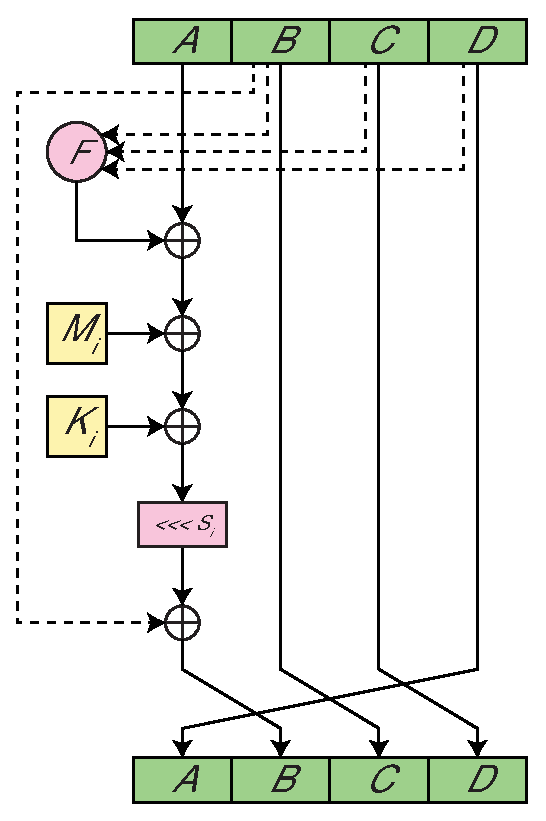
\includegraphics[width=7.5cm]{img/md5_operation.eps}
    \captionsetup{singlelinecheck=off}
    \caption[blablabla]{
    Jedna operacja \texttt{MD5}. Oznaczenia:
    \begin{itemize}
        \item $A$, $B$, $C$~i~$D$~-- wektory stanu wewnętrznego,
        \item $F$~-- funkcja rundy,
        \item $W_j$~-- $j$-ty 32-bitowy fragment pochodzący od 512-bitowego
        bloku wiadomości,
        \item $K_i$~-- 32-bitowa stała,
        \item $S_i$~-- stała oznaczająca ilość bitów w~przesunięciu cyklicznym,
        \item $i$~-- numer operacji w~kontekście funkcji kompresji ($i \in (0,
        1, \ldots, 63)$),
        \item $j$~-- numer operacji w~danej rundzie ($j \in (0, 1, \ldots,
        15)$).
    \end{itemize}
    Każda kolejna operacja używa innego zestawu stałych $K_i$ oraz $S_i$, które
    zostały opisane w~tabeli~\ref{tbl:md5_operation_const}.}
    \label{fig:md5_operation}
\end{figure}



\pagebreak
\subsubsection{\texttt{SHA-1}}
Funkcja \texttt{SHA-1}, podobnie jak funkcja \texttt{MD5}, oparta jest
o~konstrukcję Merkle-Damg\r{a}rda. Została skonstruowana przez \enn{National
Security Agency}; jej nazwa wywodzi się od \en{Secure Hash Algorithm}
(bezpieczna funkcja haszująca). \texttt{SHA-1} jest jedną z~serii funkcji
\texttt{SHA} i~choć po niej przyszły kolejne, bezpieczniejsze funkcje, to na
obecną chwilę jest najpopularniejszą funkcją z~serii \texttt{SHA}.
\texttt{SHA-1} zwraca skróty o~długości 160~bitów. Konstrukcja
funkcji~\cite{sha1_definition} została przedstawiona poniżej.

\begin{myenumerate}

    \item Faza dopełnienia bitowego: wygląda tak samo, jak faza dopełnienia
    bitowego funkcji \texttt{MD5}.

    \item Faza kompresji

    \begin{myenumerate}

        \item Wprowadzamy wewnętrzny stan, będący wektorem 160~bitów, w~którym
        wyróżniamy 5~wektorów oznaczonych kolejno: $A$, $B$, $C$, $D$ i~$E$
        (każdy o~długości 32~bitów). Wektor ten jest inicjowany wartościami na
        podstawie stałego wektora $\mathtt{IV}$:

        \[
            \begin{aligned}
                A &:= \mathtt{0x67452301} \\
                B &:= \mathtt{0xefcdab89} \\
                C &:= \mathtt{0x98badcfe} \\
                D &:= \mathtt{0x10325476} \\
                E &:= \mathtt{0xc3d2e1f0}
            \end{aligned}
        \]

        \item Dla każdego kolejnego 512-bitowego bloku wiadomości \break $M_0,
        M_1, M_2, \ldots, M_n$ aktualizujemy stan wewnętrzny funkcją kompresji,
        która przebiega w~następujący sposób:

        \begin{itemize}

            \item Podziel blok wiadomości $M_k$ na $16$ fragmentów $W_{0 \leq i
            \leq 15}$, każdy o~długości 32~bitów.

            \item Skonstruuj dodatkowe wektory $W_{16 \leq i \leq 79}$ zgodnie
            z~wzorem:

            $$
                W_i = (W_{i-3} \oplus W_{i-8} \oplus W_{i-14} \oplus W_{i-16})
                \llless 1
            $$

            \item Wykonaj 4~rundy:

            \begin{itemize}

                \item Wybierz funkcję rundy~$F$ oraz stałą rundy~$K$ zgodnie
                z~tabelą~\ref{tbl:sha1_round_function}.

                \item Wykonaj 20~operacji przekształcających stan $(A,B,C,D,E)$
                na podstawie jego poprzedniej wartości, funkcji rundy~$F$,
                stałej rundy~$K$ oraz wektorów~$W$. Konstrukcja pojedynczej
                operacji została przedstawiona na
                rysunku~\ref{fig:sha1_operation}.

            \end{itemize}

        \end{itemize}

    \end{myenumerate}

    \item Po wykonaniu wszystkich 80~operacji (4~rundy $\times$ 20~operacji),
    stan wewnętrzny $(A,B,C,D,E)$ jest zwracany jako wyjściowy skrót z~funkcji.

\end{myenumerate}

\begin{table}[H]
    \caption{Funkcja $F$ oraz stała $K$ użyta w~kolejnych rundach
    \texttt{SHA-1}.}
    \label{tbl:sha1_round_function}
    \begin{tabular}{|l|l|l|}
        \hline
        Runda & Funkcja rundy & Stała K \\
        \hline
        Runda 1 &
        $F(B,C,D) = (B \land C) \lor (\lnot B \land D)$ &
        $K = \mathtt{0x5a827999}$ \\

        Runda 2 &
        $F(B,C,D) = B \oplus C \oplus D$ &
        $K = \mathtt{0x6ed9eba1}$ \\

        Runda 3 &
        $F(B,C,D) = (B \land C) \lor (B \land D) \lor (C \land D)$ &
        $K = \mathtt{0x8f1bbcdc}$ \\

        Runda 4 &
        $F(B,C,D) = B \oplus C \oplus D$ &
        $K = \mathtt{0xca62c1d6}$ \\
        \hline
    \end{tabular}
\end{table}

\begin{figure}[H]
    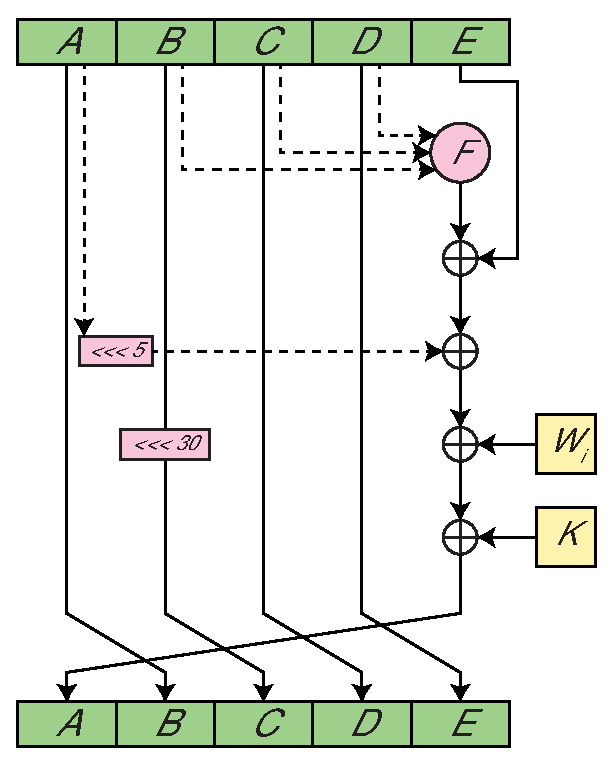
\includegraphics[width=8.5cm]{img/sha1_operation.eps}
    \captionsetup{singlelinecheck=off}
    \caption[blablabla]{
    Jedna operacja \texttt{SHA-1}. Oznaczenia:
    \begin{itemize}
        \item $A$, $B$, $C$, $D$~i~$E$~-- wektory stanu wewnętrznego,
        \item $F$~-- funkcja rundy,
        \item $K$~-- 32-bitowa stała rundy,
        \item $W_i$~-- $i$-ty 32-bitowy fragment pochodzący od rozszerzenia
        512-bitowego bloku wiadomości,
        \item $i$~-- numer operacji w~kontekście funkcji kompresji ($i \in (0,
        1, \ldots, 79)$).
    \end{itemize}}
    \label{fig:sha1_operation}
\end{figure}




\newpage
\section{Ataki uniwersalne}
\label{sec:universal_attacks}

Wprawdzie kryptograficzne funkcje haszujące z~założenia są bezpieczne, nie
oznacza to, że są one nie do złamania. Istnieje kilka ogólnych technik, które
można stosować do znajdywania oryginalnych wiadomości $m$ niezależnie od
rodzaju użytej funkcji.

\subsection{Ataki naiwne}

Wyobraźmy sobie scenariusz, w~którym z~serwera uwierzytelniającego została
wykradziona baza danych zawierająca nazwy użytkowników i~ich hasła zakodowane
dowolną funkcją haszującą. W~naiwnym podejściu atakujący może próbować zgadnąć
kolejne hasła, jakich mogli użyć użytkownicy i~porównywać hasze tych
wymyślonych haseł z~haszami z~wykradzionej bazy danych.

\subsubsection{Atak brutalny}

W~tym podejściu konsekwentnie wypróbowywane są wszystkie hasła, jakie się da
utworzyć za pomocą danego alfabetu $A$, zwiększając długość wypróbowywanych
haseł \latin{ad infinitum}. Przykładowo, mając alfabet $A=(\mathtt{a},
\mathtt{b}, \mathtt{c}, \ldots, \mathtt{z})$ atakujący będzie wypróbowywał
znaleźć kolizje haszy kolejno dla $\mathtt{a}, \mathtt{b}, \mathtt{c}, \ldots,
\mathtt{z}, \mathtt{aa}, \mathtt{ab}, \ldots$ itd.

Choć bardzo prosta, technika ta jest wyjątkowo nieoptymalna z~uwagi na ilość
zasobów, których potrzebuje do pomyślnego przeprowadzenia. Chcąc sprawdzić
wszystkie hasła długości $|m| \in (1, \ldots n)$ nad alfabetem długości
$a=|A|$, musimy przeprowadzić następującą liczbę operacji haszowania:
    $$\sum_{i=1}^n a^i = \frac{a(a^n-1)}{a-1}$$
Przykładowo, chcąc sprawdzić wszystkie hasła nad alfabetem składającym się
z~cyfr oraz z~małych i~dużych znaków alfabetu łacińskiego (a~więc $|A| =
26+26+10 = 62$) o~długości od~1~do~8~znaków, musimy wypróbować następującą
liczbę możliwości:
    $$\frac{62(62^8-1)}{62-1} = \num{221919451578090}$$
Zakładając, że potrafimy obliczyć 100000~haszy na~sekundę, nadal potrzebujemy
ok.~70~lat na złamanie hasła, jest to zatem wyjątkowo niepraktyczne podejście
i~z~reguły skazane jest na niepowodzenie.

\subsubsection{Statystyczne ataki brutalne}

Mimo że ataki brutalne w~domyślnej formie są niepraktyczne, atakujący mogą
jednak wprowadzić różnego rodzaju ulepszenia tak, by nie marnować czasu na
przeszukiwanie nieprawdopodobnych haseł. Pierwszym z~takich podejść jest
wykorzystanie zdobyczy analizy częstościowej: wiadomo, że w~pewnych językach
pewne litery są częściej wykorzystywane niż inne, a~większość osób nie stara
się czynić swoich haseł bezpiecznymi i~korzysta z~haseł będącymi zwykłymi
słowami istniejącymi w~jakimś języku (więcej
w~sekcji~\ref{sec:dictionary_attacks}).

%todo: obrazek z przykładowym wykresem częstości sporządzonym z listy 2 i 1

Można wykorzystać to na
dwojaki sposób: po pierwsze, możemy ułożyć nasz alfabet w~kolejności zgodnej
z~kolejnością występowania liter w~danym języku. Przykładowo, podczas gdy
domyślnie korzystalibyśmy z~alfabetu ułożonego w~następujący sposób:
    $$A_1 = (
    \mathtt{a}, \mathtt{b}, \mathtt{c}, \mathtt{d}, \mathtt{e}, \mathtt{f},
    \mathtt{g}, \mathtt{h}, \mathtt{i}, \mathtt{j}, \mathtt{k}, \mathtt{l},
    \mathtt{m}, \mathtt{n}, \mathtt{o}, \mathtt{p}, \mathtt{q}, \mathtt{r},
    \mathtt{s}, \mathtt{t}, \mathtt{u}, \mathtt{v}, \mathtt{w}, \mathtt{x},
    \mathtt{y}, \mathtt{z})$$
Dla języka angielskiego moglibyśmy ułożyć alfabet w~kolejności
następującej:
    $$A_2 = (
    \mathtt{e}, \mathtt{t}, \mathtt{a}, \mathtt{o}, \mathtt{i}, \mathtt{n},
    \mathtt{s}, \mathtt{h}, \mathtt{r}, \mathtt{d}, \mathtt{l}, \mathtt{c},
    \mathtt{u}, \mathtt{m}, \mathtt{w}, \mathtt{f}, \mathtt{g}, \mathtt{y},
    \mathtt{p}, \mathtt{b}, \mathtt{v}, \mathtt{k}, \mathtt{j}, \mathtt{x},
    \mathtt{q}, \mathtt{z})$$
Przypuśćmy, że hasło brzmi ``thesis'' i~szukamy go metodą brutalną. Dla
zadanego alfabetu $A$, zanim znajdziemy słowo ``thesis'' musimy wygenerować
następującą liczbę pozycji:
    \[
        \begin{aligned}
        (A[\mathtt{t}]-1)\cdot(|A|^5) &+\\
        (A[\mathtt{h}]-1)\cdot(|A|^4) &+\\
        (A[\mathtt{e}]-1)\cdot(|A|^3) &+\\
        (A[\mathtt{s}]-1)\cdot(|A|^2) &+\\
        (A[\mathtt{i}]-1)\cdot(|A|^1) &+\\
        (A[\mathtt{s}]-1)\cdot(|A|^0)
        \end{aligned}
    \]
gdzie $A[x]$ oznacza pozycję litery $x$ w~alfabecie $A$ (indeksując od 1).
Korzystając z~powyższego wzoru możemy obliczyć, ile nam zajmie znalezienie
hasła metodą brutalną z~domyślnym alfabetem $A_1$:
    \[
        \begin{aligned}
        n_1=\;&19 \cdot \num{916132832} + 7 \cdot \num{14776336}\\
        +\;&4 \cdot \num{238328} + 18 \cdot \num{3844}\\
        +\;&8 \cdot \num{62} + 18 \cdot \num{1}\\
        =\;&\num{17510981178}
        \end{aligned}
    \]
\ldots a~ile zajmie nam znalezienie hasła przy pomocy mądrze spreparowanego
$A_2$:
    \[
        \begin{aligned}
        n_2=\;&1 \cdot \num{916132832} + 7 \cdot \num{14776336}\\
        +\;&0 \cdot \num{238328} + 6 \cdot \num{3844}\\
        +\;&4 \cdot \num{62} + 6 \cdot \num{1}\\
        =\;&\num{1019590502}
        \end{aligned}
    \]
Jest to ponad 17 razy krócej. Przyrost ten głównie wynika z~dobrego wyboru
pierwszej litery.

\subsubsection{Zrandomizowane ataki brutalne}
Powyższa obserwacja prowadzi nas do innego sposobu optymalizowania szukania:
gdy przeszukujemy przestrzeń haseł liniowo, to tak naprawdę powodzenie szukania
jest najbardziej uzależnione od dobrego doboru pierwszej litery. Jest to
niepożądane zjawisko, dlatego wykształciła się inna rodzina ataków brutalnych,
jaką są ataki zrandomizowane -- zamiast liniowo przeszukiwać przestrzeń haseł,
próbujemy je przeszukiwać nieliniowo tak, by każda kombinacja miała równą
szansę być wypróbowana wraz z~upływem czasu. Wyszukiwanie nieliniowe można
zaimplementować na kilka sposobów.
\begin{myenumerate}
    \item Na pierwszy rzut oka nasuwa się myśl, że moglibyśmy po prostu
    wygenerowane hasła potasować. Podejście to jest jednak złe, ponieważ
    potasowanie odbywa się tutaj dopiero \emph{po} wygenerowaniu, a~zatem nic
    tak naprawdę nie zyskujemy, a~wręcz tracimy. Należy pamiętać, że kluczowym
    elementem jest uzyskanie losowości już podczas generowania.
    \item Możemy zmienić sposób obliczania następnika, tzn. nowego hasła na
    podstawie starego, tak by wpływał na całe hasło w~sposób jak najbliższy
    losowemu. Podejście to znajduje swoje korzenie w~trybach szyfrów blokowych,
    gdzie zazwyczaj zależy nam by poprzedni blok wpływał jak najbardziej
    nieprzewidywalny sposób na wygląd aktualnego bloku (dowolny tryb inny niż
    \texttt{ECB}). Wadą tego rozwiązania jest to, że implementacja iteratora,
    który będzie zwracał wyniki wyglądające jak losowe, jest kosztowna
    obliczeniowo, a~przy generowaniu haseł zależy nam na jak najoptymalniejszym
    szybkościowo i~pamięciowo działaniu procesu.
    \item Możemy też zwyczajnie\ldots generować przypadkowe hasła. Jest to
    podejście najlepsze, bo nie dość, że jest mało kosztowne obliczeniowo
    (zakładając szybkość działania wykorzystanych generatorów liczb
    pseudolosowych), to zostawia także dużo miejsca na kolejne ulepszenia.
\end{myenumerate}
Generowanie losowych haseł możemy zaimplementować na różne sposoby. Możemy na
przykład po prostu składać ze sobą $n$ przypadkowych znaków z~alfabetu $A$.
Popełnialibyśmy jednak w~ten sposób ten sam błąd, co wcześniej -- także i~w~tym
podejściu powinniśmy skorzystać z~dobrodziejstwa analizy~częstościowej
i~uzależnić prawdopodobieństwa wyciągnięcia odpowiednich liter od
prawdopodobieństwa ich wystąpienia w~zakładanym języku. Możemy pójść także krok
dalej i~uzależnić swój generator od prawdopodobieństw występowania tzw.
digramów oraz trigramów, czyli ciągów odpowiednio 2- i~3-literowych.
Przykładowo, w~języku angielskim najpopularniejszymi digramami są:
    \begin{center}
    \begin{BVerbatim}
    th, er, on, an, re, he, in, ed, nd, ha,
    at, en, es, of, or, nt, ea, ti, to, it,
    st, io, le, is, ou, ar, as, de, rt, ve
    \end{BVerbatim}
    \end{center}
Natomiast najczęściej występującymi trigramami są:
    \begin{center}
    \begin{BVerbatim}
    the, and, tha, ent, ion, tio, for,
    nde, has, nce, edt, tis, oft, sth
    \end{BVerbatim}
    \end{center}
%todo: zamienić to na tabelkę sporządzoną na podstawie listy 2, wraz z
%prawdopodobieństwami
Gdy usprawnimy swój generator w~ten sposób, staje się on naprawdę dobrym
narzędziem, co znajduje potwierdzenie w~popularności, jaką cieszy się program
\texttt{Johnny The Ripper} wykorzystujący powyższe techniki.



\subsubsection{Atak słownikowy}
\label{sec:dictionary_attacks}

\subsubsection{``Mutowanie'' kandydatów}

\subsubsection{Przyspieszanie obliczeń}

\subsection{Tęczowe tablice}

\subsection{Ataki typu Denial of Service}

\section{Ataki teoretyczne}

\subsection{Ataki na słabe funkcje haszujące}

\subsubsection{\en{Collision resistance}}

\subsubsection{\en{Preimage resistance}}

\subsubsection{\en{Second preimage resistance}}

\section{Podsumowanie}

\newpage
\section{Bibliografia}
\begingroup
\renewcommand{\section}[2]{}
\bibliographystyle{plain}
\bibliography{bibliography}
\endgroup

\newpage
\begin{appendices}
\section{Oznaczenia operacji bitowych}
\label{app:bitwise_operations}

    W~pracy używane są następujące oznaczenia operatorów:

    \begin{itemize}
        \item $\land$ lub $\&$~-- operator koniunkcji,
        \item $\lor$ lub $|$~-- operator alternatywy,
        \item $\oplus$~-- operator alternatywy wykluczającej.
    \end{itemize}

    \noindent Powyższe operatory przypisują dla każdej pary bitów $a$, $b$
    w~wektorach $A$~i~$B$ wartości zgodnie z~poniższą tabelą:

    \begin{center}
        \begin{tabular}{ |c|c||c|c|c| }
            \hline
            $a$ & $b$ & $a \land b$ & $a \lor b$ & $a \oplus b$ \\
            \hline
            1 & 1 & 1 & 1 & 0 \\
            1 & 0 & 0 & 1 & 1 \\
            0 & 1 & 0 & 1 & 1 \\
            0 & 0 & 0 & 0 & 0 \\
            \hline
        \end{tabular}
    \end{center}

    \noindent Ponadto wykorzystane są poniższe oznaczenia operatorów przesunięć
    ($c$ oznacza ilość bitów, którą dana zmienna jest w~stanie pomieścić).

    \begin{itemize}

        \item $\ll$~-- operator przesunięcia bitowego w~lewo. $a \ll n$ oznacza
        $a$ przesunięte w~lewo o~$n$ bitów gdzie bity, które w~wyniku
        przesunięcia wychodzą poza zakres $c$, są tracone.

        \item $\gg$~-- operator przesunięcia bitowego w~prawo. Działanie jest
        analogiczne do poprzedniego operatora.

        \item $\llless$~-- operator cyklicznego przesunięcia bitowego w~lewo.
        $a \llless n$ oznacza $a$ przesunięcie w~lewo o~$n$ bitów gdzie bity,
        które w~wyniku przesunięcia wychodzą poza zakres $c$, są dopisywane
        z~powrotem z~prawej strony; $a \llless n =\break ((a \ll n) \land
        \underbrace{111\ldots1}_{c\;\text{bitów}}) \;\lor\; (a \gg (c-n))$.

        \item $\ggg$~-- operator cyklicznego przesunięcia bitowego w~prawo.
        Działanie jest analogiczne do poprzedniego operatora.

    \end{itemize}

\section{Listy słów użyta do statystyk}
\label{app:wordlists}
W~pracy w~testach statystycznych korzystano z~kilku list.

    \begin{myenumerate}

        \item \refstepcounter{wlcounter}\label{wl:english_wordlist} Słownik
        języka angielskiego zawierający 390516 niepowtarzających się wyrazów;
        dostępny pod adresem:
        \url{http://download.openwall.net/pub/wordlists/languages/English/3-large/lower.gz}

        \item \refstepcounter{wlcounter}\label{wl:wiki_wordlist} Lista słów
        \texttt{enwik8} używana w konkursie o~Nagrodzę Huttera, stanowiąca
        pierwsze $10^8$ znaków zrzutu artykułów z~anglojęzycznej
        \mbox{Wikipedii}; dostępna pod adresem:
        \url{http://cs.fit.edu/~mmahoney/compression/enwik8.zip}. Usunięcie
        składni mediawiki oraz XML dokonane przy użyciu \texttt{WikiExtractor}
        dostepnego pod adresem:
        \url{http://medialab.di.unipi.it/wiki/Wikipedia_Extractor}.

    \end{myenumerate}

%todo: nowy dodatek zawierający zrzuty użytych programów

\end{appendices}

\end{document}
